\chapter{CMSSM}
\label{chap:CMSSM}

\section{\texttt{MasterCode framework}}
The \texttt{MasterCode} framework performs global fits following a frequentist approach. Its core consists of tools to compute the different the SUSY observables, tools to calculate the $\chi^2$ (that will be discussed in more details in \red{ref}) and the interface to an appropiate sampling algorithm, \texttt{MultiNest} \red{ref}.  
So as to compute the SUSY observables, the full MSSM spectrum for \red{electroweak observables} (including masses, mixing matrices and couplings) is computed by \texttt{SoftSUSY 3.7.2}. The Higgs sector of this spectrum is further refined using calculations from \texttt{FeynHiggs 2.10.0}. This spectrum (in a format compliant with SUSY Les Houches Accord \red{ref}) is then used as input for other codes to compute more observables and constraints, summarised in \ref{tab:MCOBS}.
From this, a global likelihood function is constructed, including contributions from electroweak precision observables, flavour measurements, the cosmological dark matter density and direct searches for dark matter, as well as the LHC Higgs mass measurement and 
$\not{E}_T$ searches. 

\begin{table}[h]
  \begin{center}
     \caption{Codes used to calculate SUSY observables in the \texttt{MasterCode} framework.}
  \begin{tabular}{|c|c|c|}
  \hline
  Code & Reference & Observables \\
    \hline
    \texttt{SoftSUSY 3.7.2} & \red{ref} & SUSY spectrum \\
    \hline
    \texttt{FeynHiggs-2.10.0} & \red{ref} & Higgs sector, $(g-2)_{\mu}$ \\
    \hline
    \texttt{micrOMEGAs-3.2} & \red{ref} & $\Omega_{\rm CDM}h^2$ \\ 
    \texttt{SSARD} & \red{ref} & $\sigma_p^{\rm SI}$, $\Delta \sigma_p^{\rm SI}$\\ 
    \texttt{SuFla}, \texttt{SuperIso v3.5} & \red{ref} & Flavour physics \\
    \texttt{FeynWZ} & \red{ref} & $M_W$, \textit{Z}-pole \\
    \hline
    \texttt{HiggsSignals-1.3.1} & \red{ref} & Constraints Higgs signal-strengths \\
    \texttt{HiggsBounds-4.2.0} & \red{ref} & Constraints $H/A \rightarrow \tau^+ \tau^-$ decay \\
    \texttt{SDECAY-1.3b} & \red{ref} & Decay tables \\
    \hline
  \end{tabular}
  \label{tab:MCOBS}
  \end{center}
\end{table}

\section{Sampling algorithm}
The main goal of the \texttt{MasterCode} framework is establishing confidence intervals for parameters and observables. In order to do this, the desired region is sampled and the likelihood function is inspected by means of the \texttt{MultiNest} algorithm \red{ref}. Even though it was designed as a Bayesian inference tool, it has proven to be very sucessful in computing profile likelihood functions \red{ref}. 

The likelihood is computed iteratively based on the so-called ellipsoidal neted sample. In this mechanism, ellipsoidal bounds are constructed in the unit cube based on clustering of N \textit{active} points. For each iteration, the point  with the lowest likelihood amongst a set of points (\textit{live} or active) is discarded, and another one with higher likelihood is searched. When found, it replaces the former, that turns into an \textit{inactive} point. This is done until the Bayesian evidence has reaches a value controled by the \textit{tolerance}.
 
Apart from its robustness and efficiency, this algorithm was specifically designed to deal with multiple local maxima and elongated curving degeneracies, thus fulfilling \texttt{MasterCode}'s requirements. A special feature of \texttt{MultiNest} is that once a point becomes active, it forms a basin of attraction, so that proximal points will be sampled. This ensures the coverage of small volumes, provided one of their points becomes active. 

In order to ensure a good coverage of the parameter space, this is divided into segments. The "cross-product" of these segments constitute \textit{boxes}. For each of these boxes, the number of active points is $N = 1000$. Priors are defined in order to convert the input parameters into physical quantities computable by the likelihood. Usually soft flat priors are used (an example of this distribution can be seen in \ref{fig:soft_prior}). With this, 80\% of the distribution lies within the nominal segment range, with the rest 20 \% lies outside these bounds. This allows for some overlap between boxes, hence avoiding edge effects between neighbouring parameter segments. 

\begin{figure} [htb!]
\begin{center}
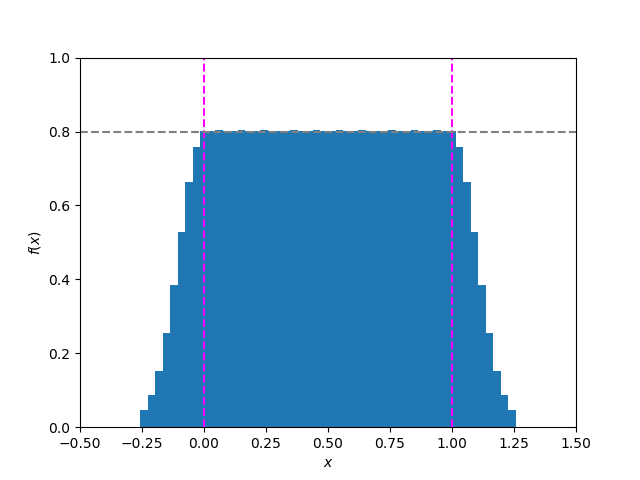
\includegraphics[scale=0.7]{figs/soft_prior.png}
\caption{Illustration of soft flat prior, for which 80\% is flat and lies within the nominal range of the segment ([0,1]), while 20\% of the distribution lies outside the nominal range, and is normally distributed. \label{fig:soft_prior}}
\end{center}
\end{figure}

\section{Scan Ranges}
The scan ranges are chosen such that they include a full coverage of parameter space, paying spacial attention to the mass scales relevant for LHC, while maintaining the Yukawa couplings perturbatively small (hence $1.2 \leqslant \tan{\beta} \geqslant 65$). The input parameters and the nuisance parameters are sampled using soft flat and Gaussian priors, respectively. The ranges, the number of segments and the resulting number of boxes that are used in the scan are given in \ref{tab:SCAN_RANGES}.

\begin{table}[h]
  \begin{center}
     \caption{Sampling ranges and segment definitions in the \red{MODEL}.}
  \begin{tabular}{|c|c|c|}
  \hline
  Parameter & Range & \# Segments \\
  \hline
  \red{MISSING} & \red{MISSING} & \red{MISSING} \\
    \hline
  \end{tabular}
  \label{tab:SCAN_RANGES}
  \end{center}
\end{table}

\section{Method}
So as to explore the different models within the \texttt{MasterCode} framework, frequentist confidence intervals and regins for the model parameters and corresponding predictions for physical observables are established. In order to do this, a $\chi^2$ function is constructed from the likelihood function using Wilks' theorem, $\chi^2 \approx -2\ln{(\theta)} + \rm const.$, being this normalisation constant irrelevant. \red{For the sake of this study}.  The $\chi^2$ function is given by
\begin{equation}
\chi^2(\theta) \equiv \sum_i \left( \frac{O_{i,\rm meas.}-O_{i,\rm pred.}}{\sigma(O_i)}\right) ^2 + \sum_j \left( \frac{\theta_{j,\rm meas.}^{\rm SM}-\theta_{j,\rm nuis.}^{\rm SM}}{\sigma(\theta_{j,\rm meas.}^{\rm SM})}\right) ^2 + \sum_k \chi^2_{k,\rm non-Gaussian}
\label{eq:MCCHI2}
\end{equation}
where $O_{i,\rm pred.}(\theta)$ ($O_{i,\rm meas.}(\theta)$)  are the predicted (measured) values for the observables, $\theta(O_i)$ is the total uncertainty, obtained adding the experimental and theoretical uncertainties in quadrature, and $\theta_{k,\rm nuis.}$ are the SM nuisance parameters {$m_t$, $\Delta \alpha_{\rm had}^{(5)}(M_Z)$, $M_Z$} that are allowed to vary in the fit while being constrained according to their measured values and uncertainties. The first two terms in \ref{eq:MCCHI2} correspond to a normal distribution of the likelihood, thus being "Gaussian" constraints, while the third tirm is "non-Gaussian" and a more refined treatment is needed. 
The confidence intervals for $n$ parameters and/or physical observables of interest at a confidence level $\alpha$ are thus given by the condition $\Delta \chi^2 \leq \Delta \chi^2(\alpha,n)$. Some typical values are given in \ref{tab:CL}.

\begin{table}[h]
  \begin{center}
     \caption{Sampling ranges and segment definitions in the \red{MODEL}.}
  \begin{tabular}{|c|c|c|}
  \hline
  $\alpha(\%)$ & $\Delta \chi^2(\alpha,1)$ & $\Delta \chi^2(\alpha,2)$ \\
  \hline
  68 & 0.99 & 2.27 \\
  68.3 & 1 & 2.30 \\
    \hline
  95 & 3.84 & 5.99 \\
  95.4 & 4 & 6.18 \\
  \hline
  99 & 6.63 & 9.21 \\
  99.7 & 9 & 11.82 \\
  \hline
  \end{tabular}
  \label{tab:CL}
  \end{center}
\end{table}

Therefore, 68\% CL intervals (regions) correspond to $\Delta\chi^2 < 1 (\Delta\chi^2 < 2.30)$, while 95\% CL intervals (regions) correspond to $\Delta\chi^2 < 4 (\Delta\chi^2 < 5.99)$ for one- (two-)dimensional profile likelihood functions. 
%we interchangeably refer to two-dmensional profile likelihood functions as "planes"

\subsection{Gaussian Constraints}
The following Gaussian Constraints are used in the study:
\begin{itemize}
\item 95\% CL lower limits on the masses of SUSY particles from ALEPH, DELPHI, L3, OPAL experiments \red{ref}.
\item Top Mass, $m_t = 173.34 \pm 0.76 \rm GeV$\red{ref}, treated as a nuisance parameter.
\item Light Higgs Boson, with a measured mass\red{ref} of $M_h = 125.09 \pm 0.24_{\rm EXP} \pm 1.5_{\rm SUSY} \rm GeV$. The assumed theoretical uncertainty for the lightest Higgs mass within MSSM (computed using \texttt{FeynHiggs-2.10.0}) is a conservative but accurate estimate of the point-by-point uncertainty that can be calculated with such \red{code}. Further constraints on the Higgs decays are incorporated using \texttt{HiggsSignals-1.3.1}. 
\item Dark Matter Relic Density, determined from anisotropies in the Cosmic Microwave Background and satellite measurements, $\Omega_{\rm CDM}h^2 = 0.1186 \pm 0.0022_{\rm EXP} \pm 0.012_{\rm TH}$, from \red{ref}. The SUSY prediction is taken from \texttt{micrOMEGAs-3.2}. Given the high sensitivity of such prediction to the given spectrum, a theoretical uncertainty of $\sim 10 \%$ is assumed.  %%%% theoretical uncertainty is much larger, the SUSY prediction is very sensitive to the MSSM spectrum. the input parameters for a given model point may need tweaking to achieve the same relic density when using different spectrum and relic density calculators 
\item The Anomalous Dipole Moment of the Muon, $(g-2)_{\mu}^{\rm EXP} - (g-2)_{\mu}^{\rm SM} = (30.2 \pm 5.4_{\rm stat} \pm 3.3_{\rm sys} \pm 6.1_{\rm SM} \pm 2.0_{\rm SUSY})\times 10^{-10}$, from \red{refs}. The anomalous dipole moment is computed within MSSM using \texttt{FeynHiggs-2.10.0}. 
\item Electroweak Precision Observables, $M_W$ and the $Z$-pole observables. These are computed using \texttt{FeynWZ}. Its inputs, $\Delta\alpha_{\rm had}^{(5)}(M_Z)$ and $M_Z$, are treated as nuisance parameters in the fit.  
\item Flavour Physics Observables, such as branching fractions from rare \textit{B} decays, rare \textit{K} decays, $B - \bar{B}$ mixing and $\epsilon_K$. The SUSY predictions for flavour physics observables are calculated using \texttt{SuFla} \red{update}.
\end{itemize}

\subsection{Non-Gaussian Constraints}
Contributions from non-Gaussian constraints include:
\begin{itemize}
\item Searches for Squarks and Gluinos by ATLAS and CMS \red{ref}, that strongly constraint the parameter space of the models. A $\chi^2$ is estrapolated from the provided contour plots. \red{ref 38 en Higgs}
\item Production of heavy neutral Higgs bosons decaying into taus, $H/A \rightarrow \tau^+ \tau^-$. As before, a $\chi^2$ is constructed from the exclusion contours from ATLAS \red{ref} and CMS \red{ref} \red{using \texttt{HiggsBounds-4.2.0}}. 
\item Spin-independent cross-section of neutralino-nucleus elastic scattering, taking into account results from LUX, XENON and PICO \red{check, refs} and theor experimental uncertainties in the theoretical calculation \red{ref 79 Kees}. 
\item \red{reinterpretation of searches?}
\end{itemize}
